%=====================================
%   2024-02-08.tex
%   院生セミナー資料 大柴寿浩
%=====================================

% -----------------------
% preamble
% -----------------------
% ここから本文 (\begin{document}) までの
% ソースコードに変更を加えた場合は
% 編集者まで連絡してください. 
% Don't change preamble code yourself. 
% If you add something
% (usepackage, newtheorem, newcommand, renewcommand),
% please tell it 
% to the editor of institutional paper of RUMS.

% ------------------------
% documentclass
% ------------------------
\documentclass[11pt, a4paper, leqno, dvipdfmx]{jsarticle}

% ------------------------
% usepackage
% ------------------------
\usepackage{algorithm}
\usepackage{algorithmic}
\usepackage{amscd}
\usepackage{amsfonts}
\usepackage{amsmath}
\usepackage[psamsfonts]{amssymb}
\usepackage{amsthm}
\usepackage{ascmac}
\usepackage{bm}
\usepackage{color}
\usepackage{enumerate}
\usepackage{fancybox}
\usepackage[stable]{footmisc}
\usepackage{graphicx}
\usepackage{listings}
\usepackage{mathrsfs}
\usepackage{mathtools}
\usepackage{otf}
\usepackage{pifont}
\usepackage{proof}
\usepackage{subfigure}
\usepackage{tikz}
\usepackage{verbatim}
\usepackage[all]{xy}

\usetikzlibrary{cd}



% ================================
% パッケージを追加する場合のスペース 
\usepackage[dvipdfmx]{hyperref}
\usepackage{xcolor}
\definecolor{darkgreen}{rgb}{0,0.45,0} 
\definecolor{darkred}{rgb}{0.75,0,0}
\definecolor{darkblue}{rgb}{0,0,0.6} 
\hypersetup{
    colorlinks=true,
    citecolor=darkgreen,
    linkcolor=darkred,
    urlcolor=darkblue,
}
\usepackage{pxjahyper}

%=================================


% --------------------------
% theoremstyle
% --------------------------
\theoremstyle{definition}

% --------------------------
% newtheoem
% --------------------------

% 日本語で定理, 命題, 証明などを番号付きで用いるためのコマンドです. 
% If you want to use theorem environment in Japanece, 
% you can use these code. 
% Attention!
% All theorem enivironment numbers depend on 
% only section numbers.
\newtheorem{Axiom}{公理}[section]
\newtheorem{Definition}[Axiom]{定義}
\newtheorem{Theorem}[Axiom]{定理}
\newtheorem{Proposition}[Axiom]{命題}
\newtheorem{Lemma}[Axiom]{補題}
\newtheorem{Corollary}[Axiom]{系}
\newtheorem{Example}[Axiom]{例}
\newtheorem{Claim}[Axiom]{主張}
\newtheorem{Property}[Axiom]{性質}
\newtheorem{Attention}[Axiom]{注意}
\newtheorem{Question}[Axiom]{問}
\newtheorem{Problem}[Axiom]{問題}
\newtheorem{Consideration}[Axiom]{考察}
\newtheorem{Alert}[Axiom]{警告}
\newtheorem{Fact}[Axiom]{事実}


% 日本語で定理, 命題, 証明などを番号なしで用いるためのコマンドです. 
% If you want to use theorem environment with no number in Japanese, You can use these code.
\newtheorem*{Axiom*}{公理}
\newtheorem*{Definition*}{定義}
\newtheorem*{Theorem*}{定理}
\newtheorem*{Proposition*}{命題}
\newtheorem*{Lemma*}{補題}
\newtheorem*{Example*}{例}
\newtheorem*{Corollary*}{系}
\newtheorem*{Claim*}{主張}
\newtheorem*{Property*}{性質}
\newtheorem*{Attention*}{注意}
\newtheorem*{Question*}{問}
\newtheorem*{Problem*}{問題}
\newtheorem*{Consideration*}{考察}
\newtheorem*{Alert*}{警告}
\newtheorem{Fact*}{事実}


% 英語で定理, 命題, 証明などを番号付きで用いるためのコマンドです. 
% If you want to use theorem environment in English, You can use these code.
%all theorem enivironment number depend on only section number.
\newtheorem{Axiom+}{Axiom}[section]
\newtheorem{Definition+}[Axiom+]{Definition}
\newtheorem{Theorem+}[Axiom+]{Theorem}
\newtheorem{Proposition+}[Axiom+]{Proposition}
\newtheorem{Lemma+}[Axiom+]{Lemma}
\newtheorem{Example+}[Axiom+]{Example}
\newtheorem{Corollary+}[Axiom+]{Corollary}
\newtheorem{Claim+}[Axiom+]{Claim}
\newtheorem{Property+}[Axiom+]{Property}
\newtheorem{Attention+}[Axiom+]{Attention}
\newtheorem{Question+}[Axiom+]{Question}
\newtheorem{Problem+}[Axiom+]{Problem}
\newtheorem{Consideration+}[Axiom+]{Consideration}
\newtheorem{Alert+}{Alert}
\newtheorem{Fact+}[Axiom+]{Fact}
\newtheorem{Remark+}[Axiom+]{Remark}

% ----------------------------
% commmand
% ----------------------------
% 執筆に便利なコマンド集です. 
% コマンドを追加する場合は下のスペースへ. 

% 集合の記号 (黒板文字)
\newcommand{\NN}{\mathbb{N}}
\newcommand{\ZZ}{\mathbb{Z}}
\newcommand{\QQ}{\mathbb{Q}}
\newcommand{\RR}{\mathbb{R}}
\newcommand{\CC}{\mathbb{C}}
\newcommand{\PP}{\mathbb{P}}
\newcommand{\KK}{\mathbb{K}}


% 集合の記号 (太文字)
\newcommand{\nn}{\mathbf{N}}
\newcommand{\zz}{\mathbf{Z}}
\newcommand{\qq}{\mathbf{Q}}
\newcommand{\rr}{\mathbf{R}}
\newcommand{\cc}{\mathbf{C}}
\newcommand{\pp}{\mathbf{P}}
\newcommand{\kk}{\mathbf{K}}

% 特殊な写像の記号
\newcommand{\ev}{\mathop{\mathrm{ev}}\nolimits} % 値写像
\newcommand{\pr}{\mathop{\mathrm{pr}}\nolimits} % 射影

% スクリプト体にするコマンド
%   例えば {\mcal C} のように用いる
\newcommand{\mcal}{\mathcal}

% 花文字にするコマンド 
%   例えば {\h C} のように用いる
\newcommand{\h}{\mathscr}

% ヒルベルト空間などの記号
\newcommand{\F}{\mcal{F}}
\newcommand{\X}{\mcal{X}}
\newcommand{\Y}{\mcal{Y}}
\newcommand{\Hil}{\mcal{H}}
\newcommand{\RKHS}{\Hil_{k}}
\newcommand{\Loss}{\mcal{L}_{D}}
\newcommand{\MLsp}{(\X, \Y, D, \Hil, \Loss)}

% 偏微分作用素の記号
\newcommand{\p}{\partial}

% 角カッコの記号 (内積は下にマクロがあります)
\newcommand{\lan}{\langle}
\newcommand{\ran}{\rangle}



% 圏の記号など
\newcommand{\Set}{{\bf Set}}
\newcommand{\Vect}{{\bf Vect}}
\newcommand{\FDVect}{{\bf FDVect}}
%\newcommand{\Ring}{{\bf Ring}}
\newcommand{\Ab}{{\bf Ab}}
\newcommand{\Mod}{\mathop{\mathrm{Mod}}\nolimits}
\newcommand{\Modf}{\mathop{\mathrm{Mod}^\mathrm{f}}\nolimits}
\newcommand{\CGA}{{\bf CGA}}
\newcommand{\GVect}{{\bf GVect}}
\newcommand{\Lie}{{\bf Lie}}
\newcommand{\dLie}{{\bf Liec}}



% 射の集合など
\newcommand{\Map}{\mathop{\mathrm{Map}}\nolimits} % 写像の集合
\newcommand{\Hom}{\mathop{\mathrm{Hom}}\nolimits} % 射集合
\newcommand{\End}{\mathop{\mathrm{End}}\nolimits} % 自己準同型の集合
\newcommand{\Aut}{\mathop{\mathrm{Aut}}\nolimits} % 自己同型の集合
\newcommand{\Mor}{\mathop{\mathrm{Mor}}\nolimits} % 射集合
\newcommand{\Ker}{\mathop{\mathrm{Ker}}\nolimits} % 核
\newcommand{\Img}{\mathop{\mathrm{Im}}\nolimits} % 像
\newcommand{\Cok}{\mathop{\mathrm{Coker}}\nolimits} % 余核
\newcommand{\Cim}{\mathop{\mathrm{Coim}}\nolimits} % 余像

% その他便利なコマンド
\newcommand{\dip}{\displaystyle} % 本文中で数式モード
\newcommand{\e}{\varepsilon} % イプシロン
\newcommand{\dl}{\delta} % デルタ
\newcommand{\pphi}{\varphi} % ファイ
\newcommand{\ti}{\tilde} % チルダ
\newcommand{\pal}{\parallel} % 平行
\newcommand{\op}{{\rm op}} % 双対を取る記号
\newcommand{\lcm}{\mathop{\mathrm{lcm}}\nolimits} % 最小公倍数の記号
\newcommand{\Probsp}{(\Omega, \F, \P)} 
\newcommand{\argmax}{\mathop{\rm arg~max}\limits}
\newcommand{\argmin}{\mathop{\rm arg~min}\limits}





% ================================
% コマンドを追加する場合のスペース 
%\newcommand{\OO}{\mcal{O}}



\renewcommand\proofname{\bf 証明} % 証明
\numberwithin{equation}{section}
\newcommand{\cTop}{\textsf{Top}}
%\newcommand{\cOpen}{\textsf{Open}}
\newcommand{\Op}{\mathop{\textsf{Open}}\nolimits}
\newcommand{\Ob}{\mathop{\textrm{Ob}}\nolimits}
\newcommand{\id}{\mathop{\mathrm{id}}\nolimits}
\newcommand{\pt}{\mathop{\mathrm{pt}}\nolimits}
\newcommand{\res}{\mathop{\rho}\nolimits}
\newcommand{\A}{\mcal{A}}
\newcommand{\B}{\mcal{B}}
\newcommand{\C}{\mcal{C}}
\newcommand{\D}{\mcal{D}}
\newcommand{\E}{\mcal{E}}
\newcommand{\G}{\mcal{G}}
%\newcommand{\H}{\mcal{H}}
\newcommand{\I}{\mcal{I}}
\newcommand{\J}{\mcal{J}}
\newcommand{\OO}{\mcal{O}}
\newcommand{\Ring}{\mathop{\textsf{Ring}}\nolimits}
\newcommand{\cAb}{\mathop{\textsf{Ab}}\nolimits}
%\newcommand{\Ker}{\mathop{\mathrm{Ker}}\nolimits}
\newcommand{\im}{\mathop{\mathrm{Im}}\nolimits}
\newcommand{\Coker}{\mathop{\mathrm{Coker}}\nolimits}
\newcommand{\Coim}{\mathop{\mathrm{Coim}}\nolimits}
\newcommand{\rank}{\mathop{\mathrm{rank}}\nolimits}
\newcommand{\Ht}{\mathop{\mathrm{Ht}}\nolimits}
\newcommand{\supp}{\mathop{\mathrm{supp}}\nolimits}
\newcommand{\colim}{\mathop{\mathrm{colim}}}
\newcommand{\Tor}{\mathop{\mathrm{Tor}}\nolimits}

\newcommand{\cat}{\mathscr{C}}

\newcommand{\scA}{\mathscr{A}}
\newcommand{\scB}{\mathscr{B}}
\newcommand{\scC}{\mathscr{C}}
\newcommand{\scD}{\mathscr{D}}
\newcommand{\scE}{\mathscr{E}}
\newcommand{\scF}{\mathscr{F}}
\newcommand{\scN}{\mathscr{N}}
\newcommand{\scO}{\mathscr{O}}
\newcommand{\scV}{\mathscr{V}}


\newcommand{\ibA}{\mathop{\text{\textit{\textbf{A}}}}}
\newcommand{\ibB}{\mathop{\text{\textit{\textbf{B}}}}}
\newcommand{\ibC}{\mathop{\text{\textit{\textbf{C}}}}}
\newcommand{\ibD}{\mathop{\text{\textit{\textbf{D}}}}}
\newcommand{\ibE}{\mathop{\text{\textit{\textbf{E}}}}}
\newcommand{\ibF}{\mathop{\text{\textit{\textbf{F}}}}}
\newcommand{\ibG}{\mathop{\text{\textit{\textbf{G}}}}}
\newcommand{\ibH}{\mathop{\text{\textit{\textbf{H}}}}}
\newcommand{\ibI}{\mathop{\text{\textit{\textbf{I}}}}}
\newcommand{\ibJ}{\mathop{\text{\textit{\textbf{J}}}}}
\newcommand{\ibK}{\mathop{\text{\textit{\textbf{K}}}}}
\newcommand{\ibL}{\mathop{\text{\textit{\textbf{L}}}}}
\newcommand{\ibM}{\mathop{\text{\textit{\textbf{M}}}}}
\newcommand{\ibN}{\mathop{\text{\textit{\textbf{N}}}}}
\newcommand{\ibO}{\mathop{\text{\textit{\textbf{O}}}}}
\newcommand{\ibP}{\mathop{\text{\textit{\textbf{P}}}}}
\newcommand{\ibQ}{\mathop{\text{\textit{\textbf{Q}}}}}
\newcommand{\ibR}{\mathop{\text{\textit{\textbf{R}}}}}
\newcommand{\ibS}{\mathop{\text{\textit{\textbf{S}}}}}
\newcommand{\ibT}{\mathop{\text{\textit{\textbf{T}}}}}
\newcommand{\ibU}{\mathop{\text{\textit{\textbf{U}}}}}
\newcommand{\ibV}{\mathop{\text{\textit{\textbf{V}}}}}
\newcommand{\ibW}{\mathop{\text{\textit{\textbf{W}}}}}
\newcommand{\ibX}{\mathop{\text{\textit{\textbf{X}}}}}
\newcommand{\ibY}{\mathop{\text{\textit{\textbf{Y}}}}}
\newcommand{\ibZ}{\mathop{\text{\textit{\textbf{Z}}}}}

\newcommand{\ibx}{\mathop{\text{\textit{\textbf{x}}}}}

%\newcommand{\Comp}{\mathop{\mathrm{C}}\nolimits}
%\newcommand{\Komp}{\mathop{\mathrm{K}}\nolimits}
%\newcommand{\Domp}{\mathop{\mathsf{D}}\nolimits}%複体のホモトピー圏
%\newcommand{\Comp}{\mathrm{C}}
%\newcommand{\Komp}{\mathrm{K}}
%\newcommand{\Domp}{\mathsf{D}}%複体のホモトピー圏

\newcommand{\Comp}{\mathop{\mathrm{C}}\nolimits}
\newcommand{\Komp}{\mathop{\mathsf{K}}\nolimits}
\newcommand{\Domp}{\mathop{\mathsf{D}}\nolimits}
\newcommand{\Kompl}{\mathop{\mathsf{K}^\mathrm{+}}\nolimits}
\newcommand{\Kompu}{\mathop{\mathsf{K}^\mathrm{-}}\nolimits}
\newcommand{\Kompb}{\mathop{\mathsf{K}^\mathrm{b}}\nolimits}
\newcommand{\Dompl}{\mathop{\mathsf{D}^\mathrm{+}}\nolimits}
\newcommand{\Dompu}{\mathop{\mathsf{D}^\mathrm{-}}\nolimits}
\newcommand{\Dompb}{\mathop{\mathsf{D}^\mathrm{b}}\nolimits}
\newcommand{\Dompbf}{\mathop{\mathsf{D}_\mathrm{f}^\mathrm{b}}\nolimits}




\newcommand{\CCat}{\Comp(\cat)}
\newcommand{\KCat}{\Komp(\cat)}
\newcommand{\DCat}{\Domp(\cat)}%圏Cの複体のホモトピー圏
\newcommand{\HOM}{\mathop{\mathscr{H}\hspace{-2pt}om}\nolimits}%内部Hom
\newcommand{\RHOM}{\mathop{\mathrm{R}\hspace{-1.5pt}\HOM}\nolimits}

\newcommand{\muS}{\mathop{\mathrm{SS}}\nolimits}
\newcommand{\RG}{\mathop{\mathrm{R}\hspace{-0pt}\Gamma}\nolimits}
\newcommand{\RHom}{\mathop{\mathrm{R}\hspace{-1.5pt}\Hom}\nolimits}
\newcommand{\Rder}{\mathrm{R}}

\newcommand{\simar}{\mathrel{\overset{\sim}{\rightarrow}}}%同型右矢印
\newcommand{\simarr}{\mathrel{\overset{\sim}{\longrightarrow}}}%同型右矢印
\newcommand{\simra}{\mathrel{\overset{\sim}{\leftarrow}}}%同型左矢印
\newcommand{\simrra}{\mathrel{\overset{\sim}{\longleftarrow}}}%同型左矢印

\newcommand{\hocolim}{{\mathrm{hocolim}}}
\newcommand{\indlim}[1][]{\mathop{\varinjlim}\limits_{#1}}
\newcommand{\sindlim}[1][]{\smash{\mathop{\varinjlim}\limits_{#1}}\,}
\newcommand{\Pro}{\mathrm{Pro}}
\newcommand{\Ind}{\mathrm{Ind}}
\newcommand{\prolim}[1][]{\mathop{\varprojlim}\limits_{#1}}
\newcommand{\sprolim}[1][]{\smash{\mathop{\varprojlim}\limits_{#1}}\,}

\newcommand{\Sh}{\mathrm{Sh}}
\newcommand{\PSh}{\mathrm{PSh}}

\newcommand{\rmD}{\mathrm{D}}

\newcommand{\Lloc}[1][]{\mathord{\mathcal{L}^1_{\mathrm{loc},{#1}}}}
\newcommand{\ori}{\mathord{\mathrm{or}}}
\newcommand{\Db}{\mathord{\mathscr{D}b}}

\newcommand{\codim}{\mathop{\mathrm{codim}}\nolimits}



\newcommand{\gld}{\mathop{\mathrm{gld}}\nolimits}
\newcommand{\wgld}{\mathop{\mathrm{wgld}}\nolimits}











%================================================
% 自前の定理環境
%   https://mathlandscape.com/latex-amsthm/
% を参考にした
\newtheoremstyle{mystyle}%   % スタイル名
    {5pt}%                   % 上部スペース
    {5pt}%                   % 下部スペース
    {}%              % 本文フォント
    {}%                  % 1行目のインデント量
    {\bfseries}%                      % 見出しフォント
    {.}%                     % 見出し後の句読点
    {12pt}%                     % 見出し後のスペース
    {\thmname{#1}\thmnumber{ #2}\thmnote{{\hspace{2pt}\normalfont (#3)}}}% % 見出しの書式

\theoremstyle{mystyle}
\newtheorem{AXM}{公理}[section]
\newtheorem{DFN}[AXM]{定義}
\newtheorem{THM}[AXM]{定理}
\newtheorem*{THM*}{定理}
\newtheorem{PRP}[AXM]{命題}
\newtheorem{LMM}[AXM]{補題}
\newtheorem{CRL}[AXM]{系}
\newtheorem{EG}[AXM]{例}
\newtheorem*{EG*}{例}
\newtheorem{RMK}[AXM]{注意}
\newtheorem{CNV}[AXM]{約束}
\newtheorem{CMT}[AXM]{コメント}
\newtheorem{NTN}[AXM]{記号}

% 定理環境ここまで
%====================================================

\usepackage{framed}
\definecolor{lightgray}{rgb}{0.75,0.75,0.75}
\renewenvironment{leftbar}{%
  \def\FrameCommand{\textcolor{lightgray}{\vrule width 4pt} \hspace{10pt}}% 
  \MakeFramed {\advance\hsize-\width \FrameRestore}}%
{\endMakeFramed}
\newenvironment{redleftbar}{%
  \def\FrameCommand{\textcolor{lightgray}{\vrule width 1pt} \hspace{10pt}}% 
  \MakeFramed {\advance\hsize-\width \FrameRestore}}%
 {\endMakeFramed}


% =================================





% ---------------------------
% new definition macro
% ---------------------------
% 便利なマクロ集です

% 内積のマクロ
%   例えば \inner<\pphi | \psi> のように用いる
\def\inner<#1>{\langle #1 \rangle}

% ================================
% マクロを追加する場合のスペース 

%=================================





% ----------------------------
% documenet 
% ----------------------------
% 以下, 本文の執筆スペースです. 
% Your main code must be written between 
% begin document and end document.
% ---------------------------

\title{2024/02/08 セミナー資料}
\author{大柴寿浩}
\date{}
\begin{document}
\maketitle


\section{コホモロジー構成可能層}
\subsection{理想複体}
\(A\)を可換環とする.
\(M\in\Dompb(A)\coloneqq \Dompb(\Mod(A))\)を\(A\)加群の導来圏の対象とする.
\(M\)が\textbf{理想対象}\footnote{
    \cite{Ue}による訳にしたがった.
    定訳は未だ無いと思われる.
} (perfect object) であるとは,
有限生成射影的\(A\)加群の有界複体と擬同型であることをいう.

\begin{PRP}[{\cite[Exercise I.30]{KS90}}]
    \(A\)を可換環とする.
    \begin{enumerate}[(i)]\setlength{\leftskip}{2zw}
        \item \(X\to Y\to Z\underset{+1}{\to}\)が\(\Dompb(A)\)における
        完全三角で,\(X\)と\(Y\)が理想的ならば,\(Z\)も理想的である.
        \item 理想対象の直和因子も理想対象である.
        \item \(M\in\Dompb(A)\)を理想対象とする.
        \(M^\ast\coloneqq \RHom_A(M,A)\)とおく.
        \(M^\ast\)は理想対象であり,
        標準的な射\(M\to M^{\ast\ast}\)は同型である.
    \end{enumerate}

    \(A\)がネーター環で大域次元が有限であるとする.
    \begin{enumerate}[(i)]\setcounter{enumi}{3}\setlength{\leftskip}{2zw}
        \item \(\Modf(A)\)の導来圏\(\Dompb(\Modf(A))\)の
        任意の対象は理想的である.
        \item \(\Dompbf(A)\)で各コホモロジーが\(\Modf(A)\)に
        属す対象の導来圏を表す.
        \(\Dompb(\Modf(A))\to\Dompbf(\Mod(A))\)は圏同値である.\(\blacksquare\)
    \end{enumerate}
\end{PRP}   
証明は略.

擬連接かつtor次元が有限であることと同値らしい.(\cite[lem 15.74.2]{SP})







































\section{\(\gamma\)位相}

\paragraph{錐(体)}
\cite{KS90}に錐の定義が書いてなかったのでまとめておく.
\cite{BouTVS,Mo76}を参考にした.
\begin{DFN}
    \(n\)次元実ベクトル空間\(V\)の部分集合\(\gamma\)が次の条件をみたすとき,
    \textbf{錐(あるいは錐体)}(cone) であるという.
    \[
        \text{任意の実数\(t>0\)に対し,}v\in \gamma\Longrightarrow tv\in\gamma.
    \]
\end{DFN}

\begin{CMT}
    \cite{Mo76}では\(\gamma\ne 0\)も課している.
    空集合は錐である.
    \[
        \gamma=\left\{
            (x_1,x2)\in\rr^2; 0<\arg(x_1,x_2)<7\pi/4
            \right\}
    \]
    は錐である.(図\ref{fig:cone-example}).
\end{CMT}

\begin{figure}[htb]
    \centering
    \scalebox{0.8}{
        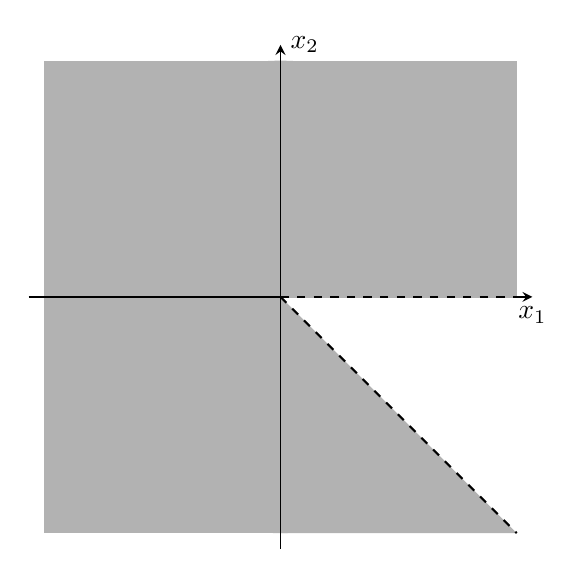
\begin{tikzpicture}[x=1cm]
            \fill [fill=black!30](0,0)--(3,0)--(3,0)arc(0:315:3)--cycle;
%                \fill[black!10] (0.7,0.1) (0,0) ellipse (2 and 2);
%            \draw[dashed,black!100] (0.7,0.1) (0,0) ellipse (2 and 2);
        \fill[black!30] (-3,3) rectangle (3,0);
        \fill[black!30] (-3,0) rectangle (0,-3);
        \fill[black!30] (0,0)--(0,-3)--(3,-3)--cycle;
        \draw[->,>=stealth,semithick] (-3.2,0)--(3.2,0)node[below]{$x_1$}; %x軸
        \draw[->,>=stealth,semithick] (0,-3.2)--(0,3.2)node[right]{$x_2$}; %y軸
        %\draw[thick] (-2,0)--(2,0); %
        \draw[dashed, thick] (0,0)--(3,-3);
        \draw[black!30,thick] (0,0)--(3,0);
        \draw[dashed, thick] (0,0)--(3,0);
%            \draw[thick] (-2,-0.2) node[left]{\(a\)};
%            \draw[thick] (2,-0.2) node[right]{\(b\)};
%            \draw (-1.3,0.1) node[above]{$F$};
%            \draw (1.3,-1) node[left]{$U$};

        %\fill[black!100](2,0) ellipse (0.1 and 0.1);
        %\draw (2,0) ellipse (0.1 and 0.1);

        %\fill[black!100](-2,0) ellipse (0.1 and 0.1);
        %\draw (-2,0) ellipse (0.1 and 0.1);
    \end{tikzpicture}}
    \caption{錐の例}
    \label{fig:cone-example}
\end{figure}
次の例を見ると,有界でないことが大事っぽい.
\begin{EG}
    \(
        \gamma\coloneqq\left\{
            (x_1,x_2)\in\rr^2;
            0<\arg(x_1,x_2)<\pi/3, 
            \lVert(x_1,x_2)\rVert<1
        \right\}
    \)
    は錐ではない.(図\ref{fig:cone-non-example})
\end{EG}

\begin{figure}[htb]
    \centering
    %\scalebox{0.8}{
        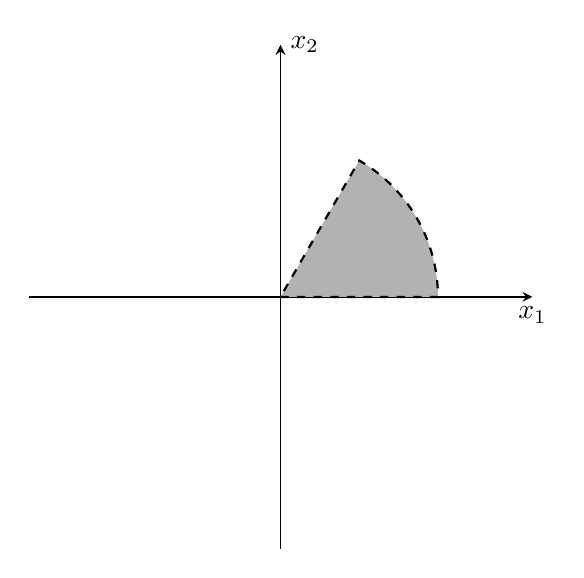
\begin{tikzpicture}[x=1cm]
        \draw[->,>=stealth,semithick] (-3.2,0)--(3.2,0)node[below]{$x_1$}; %x軸
        \draw[->,>=stealth,semithick] (0,-3.2)--(0,3.2)node[right]{$x_2$}; %x軸
        \fill [draw=black,dashed,thick, fill=black!30](0,0)--(2,0)--(2,0)arc(0:60:2)--cycle;
    \end{tikzpicture}%}
    \caption{錐でない例}
    \label{fig:cone-non-example}
\end{figure}

\begin{DFN}
    閉凸錐は閉集合で凸集合な錐.
\end{DFN}































%===============================================
% 参考文献スペース
%===============================================
\begin{thebibliography}{20} 
    \bibitem[BouTVS]{BouTVS} ブルバキ, 位相線形空間1, 東京図書, 1968.
    \bibitem[B+84]{B+84} Borel, 
    \textit{Intersection Cohomology}, 
    Progress in Mathematics, 50, Birkh\"auser, 1984.
\bibitem[G58]{G58} Grauert, 
    \textit{On Levi's problem and the embedding of real analytic manifolds}, 
    Ann. Math. 68, 460--472 (1958).
\bibitem[GP74]{GP74} Victor Guillemin, Alan Pollack, 
    \textit{Differential Topology}, 
    Prentice-Hall, 1974.
\bibitem[KS90]{KS90} Masaki Kashiwara, Pierre Schapira, 
    \textit{Sheaves on Manifolds}, 
    Grundlehren der Mathematischen Wissenschaften, 292, Springer, 1990.
\bibitem[KS06]{KS06} Masaki Kashiwara, Pierre Schapira, 
    \textit{Categories and Sheaves}, 
    Grundlehren der Mathematischen Wissenschaften, 332, Springer, 2006.
    \bibitem[Le13]{Le13} John M. Lee, 
    \textit{Introduction to Smooth Manifolds}, Second Edition,
    Graduate Texts in Mathematics, \textbf{218}, Springer, 2013.
    \bibitem[Mo76]{Mo76} 森本光生, 佐藤超函数入門, 共立出版, 1976. 
\bibitem[R55]{R55} de Rham, 
    \textit{Vari\'et\'es diff\'erentiables}, 
    Hermann, Paris, 1955.
\bibitem[Sa59]{Sa59} Mikio Sato, 
    \textit{Theory of Hyperfunctions}, 
    1959--60.
\bibitem[S66]{S66} Schwartz, 
    \textit{Th\'eorie de distributions}, 
    Hermann, Paris, 1966.
\bibitem[Sh16]{Sh16} 志甫淳, 層とホモロジー代数, 共立出版, 2016.
\bibitem[SP]{SP} The Stacks Project.
\bibitem[Sp65]{Sp65} Michael Spivak, 
\textit{Calculus on Manifolds}, 
Benjamin, 1965.
\bibitem[Ike21]{Ike21} 池祐一, 超局所層理論概説, 2021.
\bibitem[Tak17]{Tak17} 竹内潔, \(\D\)加群, 共立出版, 2017.
\bibitem[Ue]{Ue} 植田一石, ホモロジー的ミラー対称性, \url{https://www.ms.u-tokyo.ac.jp/~kazushi/course/hms.pdf} 2024/02/04 最終閲覧.

\end{thebibliography}

%===============================================


\end{document}
